\documentclass{article}
\usepackage[left=3cm,top=3cm,bottom=3cm,right=3cm]{geometry}

\documentclass[12pt,oneside,reqno]{amsart}

\usepackage{siunitx} % Provides the \SI{}{} and \si{} command for typesetting SI units

\usepackage{graphicx} % Required for the inclusion of images

\usepackage{tabularx} % Tables

\usepackage{natbib} % Required to change bibliography style to APA

\usepackage{amsmath} % Required for some math elements

\usepackage{multicol} % additional itemization formatting

% Many options for pseudocode
\usepackage{algorithm2e}
\usepackage{algorithmic}

\usepackage{listings} % Python code blocks

\usepackage{comment}

\setlength\parindent{0pt} % Removes all indentation from paragraphs

\title{Lab \#3 Report: Wall Follower on Racecar} % Title
\author{Team \#4 \\\\ Marisa Hoosen \\ Frank Gonzalez \\ Toomas Tennisberg \\ Zoe Wong \\ Kaitlin Zareno \\\\ RSS 6.141} % Team # + Names, Class (RSS)

\date{\today} % Date for the report

\begin{document}

\maketitle
\begin{comment}
(no more than 4500 words total, not including Lessons Learned; each team member should contribute approximately equal amounts to the writing of this report)\\

\textbf{Audience}\\\\
RSS faculty and staff, hypothetical managers, and professionals in the field (including your potential employers).\\

\textbf{Purpose}\\\\
Write a persuasive argument demonstrating to faculty that you understand the Lab content and how it fits into the context of the class, and that the algorithmic solution you designed is sound and works well in experiments or simulations.  Make claims for your work, supported by detailed technical explanation, justification, and experimental analysis that would be persuasive to a hypothetical manager unfamiliar with the Lab.\\

\textbf{Rubric}\\\\
See “Rubric for reports” on Canvas (Modules section).\\

\textbf{Visuals}\\\\
All visual support (graphs, charts, images, clips, tables, etc.) must be numbered, titled, captioned, and cross-referenced in-text. See the "Formatting examples for figures, pseudocode, etc" section below for examples on how to do this using LaTeX.\\

\textbf{Style}\\\\
You can modify your report to make it visually compelling, bearing in mind that ease of reading is a paramount consideration.\\

\textbf{Other}\\\\
Label each section with the author’s name.\\\\
Technical grades will be team-based; CI grades will be individual.\\\\
You may peer review each other’s sections for the purpose of learning from each other.\\\\
The report as a whole should be edited for consistency and clarity; the editor’s name should appear at the top, and editing tasks should be shared over all the Reports.\\

\textbf{Required Sections}\\\\
Use the outline of numbered sections below, not including the one on formatting examples - if using LaTeX, you can make a copy of this .tex document and fill in the blanks.
\end{comment}

\section{Introduction}
Written By: Toomas Tennisberg\\

\begin{comment}
Motivates and contextualizes this lab’s goals (i.e., identifies \textbf{what} you have designed in this lab and \textbf{how} that fits among the other RSS labs or how it contributes to developing an autonomous system). Presents an overview of the \textbf{purpose} and \textbf{specifications} of this lab. Provides a short and informal summary of the \textbf{technical problem} and introduces a bird’s-eye view of your technical solution.\\\\
(no more than 500 words)\\\\
\end{comment}

For this lab, we implemented a wall follower and safety stop mechanism for our racecar. These components are useful since autonomous navigation is required for any mobile autonomous system, while the safety stop is required to make sure that the robot does not crash into anything or anyone, which given the size and cost of the robot, would have nontrivial consequences.\\\\
The wall follower had to be able to follow a wall without crashing into it or exhibiting oscillatory behaviour. The safety stop mechanism had to sense a dangerous situation and stop the robot before a collision occurred.\\\\
Following the wall is a challenging task. The robot needs to determine the location of the wall, use that information to determine how far away it is from the wall and at what angle, and finally determine at what angle to steer the vehicle. The safety controller has to determine how far the racecar is from objects ahead of it and then determine when to stop. At the same time, it must not interfere with the normal operations of the robot.\\\\
Our solution to these challenges was to implement a modified PD controller for wall following. In addition to normal PD, it looks ahead to see if a wall is coming up and uses those data points to start turning along the perceived corner. The safety stop simply detects if enough points ahead of the car are too close, and stops the car completely if that is the case. 

\section{Technical Approach}
\begin{comment}
Formally presents the \textbf{technical problem} you have to solve in the lab.\\\\
Describes your team’s \textbf{initial set-up}, \textbf{technical approach}, and \textbf{ROS implementation}. Discusses the different building blocks of your technical approach.\\\\
Introduces required mathematical symbols and reports key mathematical relations to present the approach.\\\\
In addition to reporting on the \textbf{technical solution} you devised in response to the technical problem posted in this lab, this section explains the \textbf{how} of your approach, and should \textbf{justify} your team’s design choices and the rationale behind any tradeoffs. (Why these and not other choices?)\\\\
Any subsection must be numbered and start with a high-level overview that orients the reader.\\\\
Finally, remember to use figures to help the reader understand your approach.\\\\
(no more than 2250 words)
\end{comment}

Our main challenges for this lab were the design of a safety controller and the choice of which wall following algorithm to use on the car.

\subsection{Wall Follower}
\subsubsection{Selection Motivation}
Written By: Toomas Tennisberg\\

Coming in to this lab, all five of us had a wall follower of some sort. They were all variations of PD control with two major areas of variation.\\\\
The first variation was the value taken in as the derivative. Only one controller was implemented as the difference between two distance measurements divided by the time between them. Most other controllers calculated the change of the distance to the wall by multiplying the velocity of the robot with the sine of the angle of the robot with respect to the wall. One controller just took the angle directly and tried to minimize the angle with its steering.\\\\
The other difference to note is that some controllers had explicit corner detection: when the racecar detected a wall straight ahead, it assumed the wall was part of a corner, and started to turn immediately. This allowed the car to steer along the corner earlier and avoid crashing into the wall.\\\\
We selected Frank's controller to be the basis of our physical wall follower. Frank's controller uses velocity scaled by cosine to calculate the derivative of the error, and included corner detection by reading the points that constitute the front 30 degrees of the scanned points. It detects a wall on its side by reading a 95 degree segment centered at $\pm$49.7 degrees, depending on the robot's side. After filtering a few points out, it uses linear regression to determine the location of the wall.\\\\
Our selection was based on taking the algorithm with the best performance out of the subset of algorithms that worked both in simulation and on the actual hardware.

\subsubsection{Algorithm Overview}
Written by: Kaitlin Zareno\\

The main objective of this lab was to have our car follow a wall while maintaining a specific distance away from the wall at all times. In order to fulfill this objective, we broke down the problem into the following parts:
\begin{itemize}
  \item Obtaining and using the LaserScan data to get the relative location of the car and its surroundings
  \item Creating an internal/visual representation of the wall we want to follow from the LaserScan data
  \item Creating the PD controller that would allow the car to follow the wall
  \item Detecting whether the car should follow a straight wall or turn a corner
\end{itemize}
By partitioning our problem into these 4 modules, we were able to successfully meet our objective while reducing our error. \\ 

We discuss the more detailed implementation of these sections in the subsections below.

\subsubsection{Scan Data}
Written by: Kaitlin Zareno\\

The LaserScan data from the LIDAR sensor allowed us to obtain an array of distances which we  used to solve the problem statement. These distances describe the distance from the LIDAR sensor to the objects in its field of view. The car's field of view can be visualized Figure 1, with the first value at element 0 corresponding to the right-most datapoint in the car's field of view and the last element (99) corresponding to the left-most datapoint in the car's field of view. \\

\begin{figure}[h]
\begin{center}
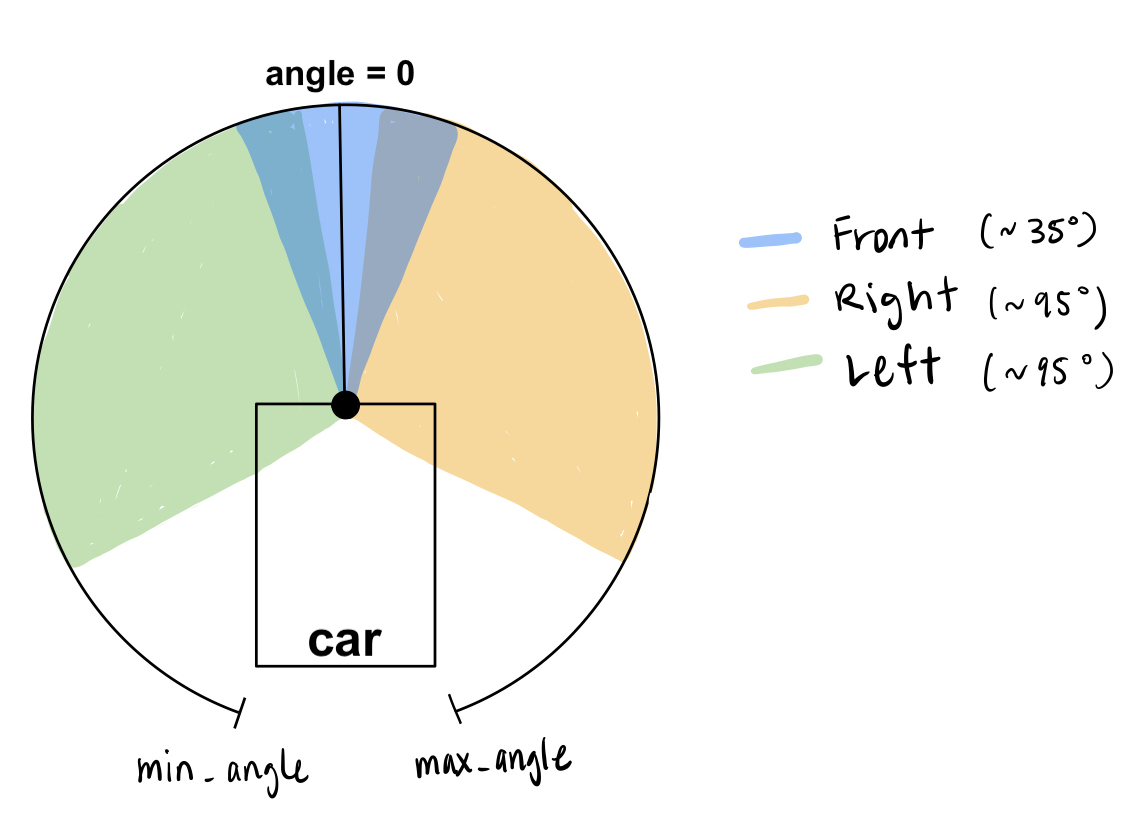
\includegraphics[width=0.5\textwidth]{imgs/IMG_0304.jpg} % Include the image
\caption{The figure illustrates the car's field of view and the slicing of the scan data.}
\end{center}
\end{figure}

The LaserScan data was split into 3 sub-arrays to account for different use cases of the data. We had a "left" subarray to account for the points on left hand side (LHS) of the car, which was necessary if we wanted the LHS of the car to follow an adjacent wall, as well as a "right" subarray, which was necessary if we wanted the right hand side (RHS) of the car to follow a wall. As indicated in the image above, each "side" subarray defined a 95 degree segment whose midpoint was at a 40.3 degree angle from 0 (straight ahead). Lastly, we had a "front" subarray which would account for any walls directly in front of the car, which we used to indicate the detection of a corner. As indicated in the image above, the "front" subarray defined a 30 degree segment that was centered at angle 0. Once we had determined what side of the car we wanted to follow the wall, we used the scan data that corresponded to that specific side to create a linear regression line that defined the wall we wanted to follow. 

\subsubsection{Linear Regression Implementation}
Written by: Kaitlin Zareno\\

From our relevant LaserScan data, we created a weighted linear regression line that represented the adjacent wall we wanted to follow. In order to do this, we first needed to interpolate the data points. Interpolating our data points allowed us to weed out outliers, which would have made our linear regression less accurate by changing the slope of the line. By removing outliers, we avoid drastic changes to the slope of our regression line that would not accurately represent the real wall, allowing us to follow it. Outliers in this case were defined as data points that existed within our subsection of LaserScan data that were greater than 1.5 times the desired distance between our car and the wall. \\

After removing the outliers from our slice of data, we converted these data points into Cartesian Coordinates relative to the car with the LIDAR scanner centered at (0,0). From these coordinates, we created a metric to ensure that points closer to the car would affect the slope of the line more than points farther away. The metric consisted of weighting the points based on their relative distance to the car and was calculated by $weight = \frac{1}{r^3}$ with $r$ being the Euclidean distance from the car to a specific Cartesian Coordinate from our scan data. Then, the coordinates and their relative weights were passed into np.polyfit() to give us a linear regression line that would "project" the wall. From this linear regression line, we were able to visualize the wall in RViz by publishing the line as a Marker, which was helpful for simulation and hardware debugging purposes. Furthermore, this "wall line" gave us the ability to create a PD controller that tracked a line parallel to the wall, allowing the car to follow the wall.

\subsubsection{PD Controller Implementation}
Written By: Frank Gonzalez\\

Now that the we had an estimate for the wall location, a PD controller was used to follow the projection. The controller was composed of two components: the error and the error's derivative. The error was calculated as the difference between the car's estimated distance to the wall and our desired distance from the wall. The derivative of the error was computed by scaling the velocity of the car by the cosine of the angle between the car's velocity vector, and the vector formed between the car and the closest point in the wall estimation. This corresponds to taking the velocity component perpendicular to the wall, which directly corresponds to the error's derivative. Figure 2 provides a geometrical view of this velocity decomposition. Both quantities were then scaled by their respective gains, and summed to calculate the steering angle. 

\begin{figure}[h]
\begin{center}
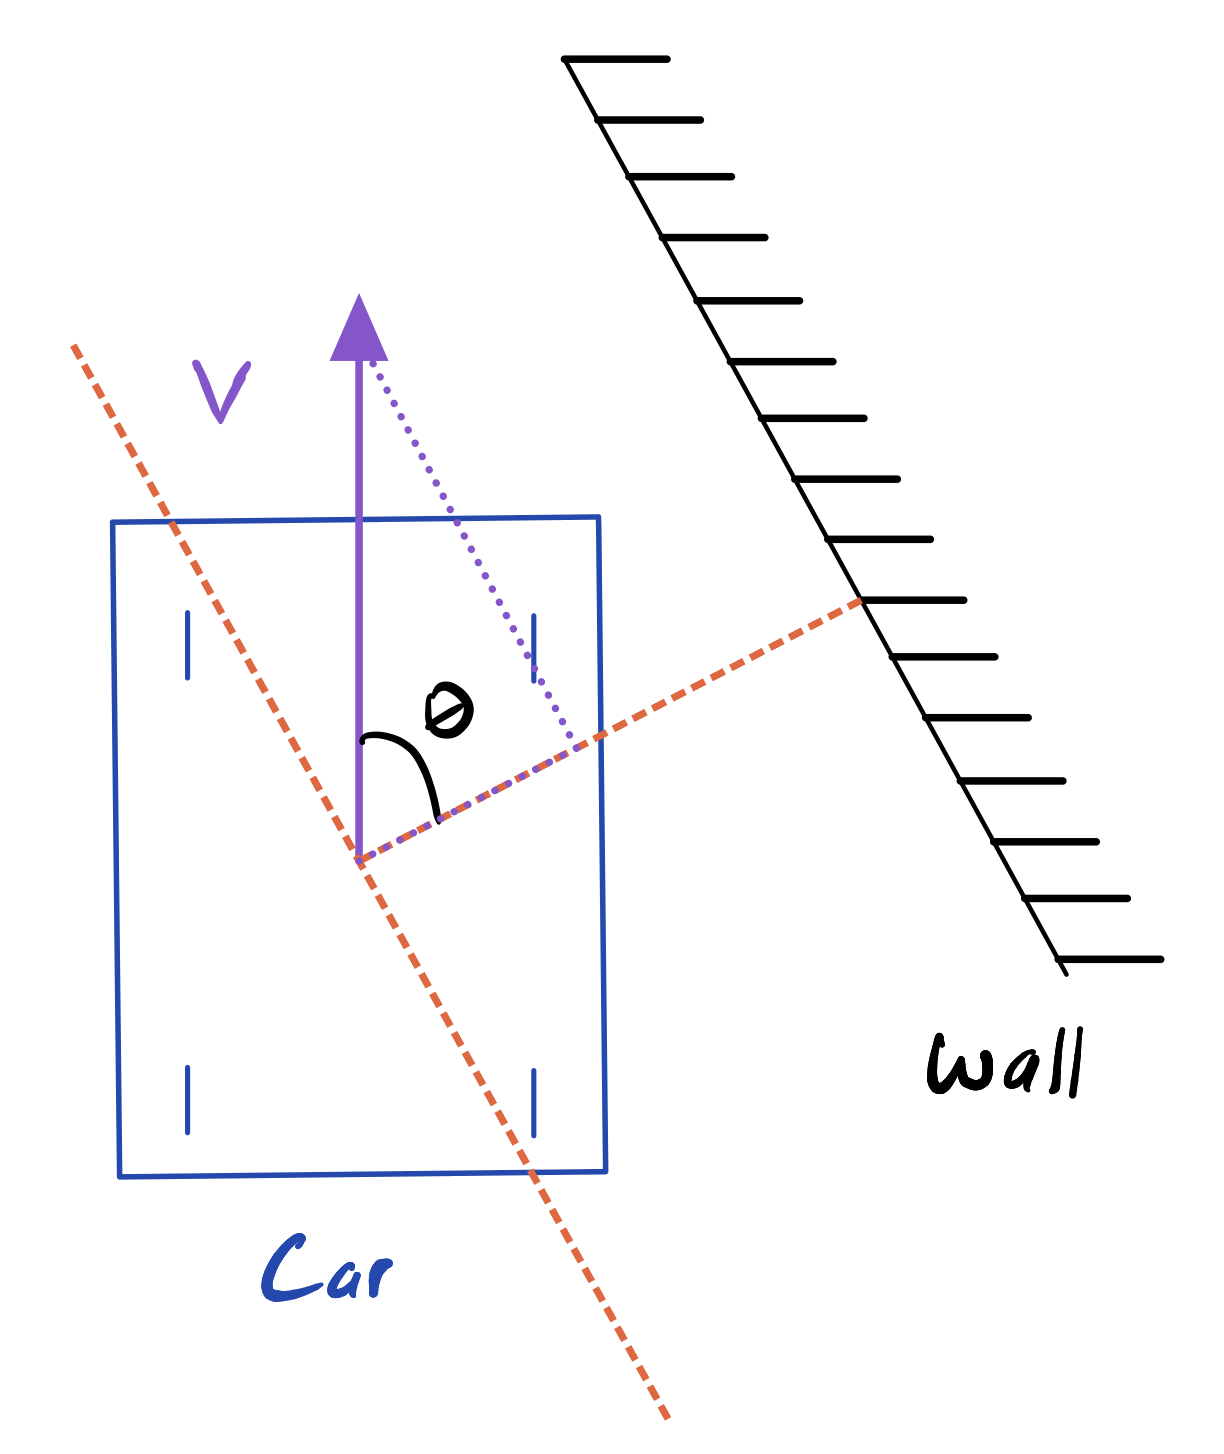
\includegraphics[width=0.5\textwidth]{imgs/velocity_decomposition.png} % Include the image
\caption{The following figure illustrates the frame in which the velocity vector is decomposed to obtain the perpendicular velocity component.}
\end{center}
\end{figure}

In order to choose the gains for the controller, the car was tuned by loosely following the Ziegler-Nichols method at 1 {m/s}. This method first involved finding the ultimate gain, $K_u$. The ultimate gain is the gain that causes the car to stably oscillate around its desired distance when only controlled with a proportional controller. The period of this oscillation was recorded as $T$. Finally, $K_p$ and $K_d$ were set according to Equations 1-4:

\begin{equation}
    K_u = 3.5
\end{equation}

\begin{equation}
    K_p = 0.4K_u
\end{equation}

\begin{equation}
    T = 7/6
\end{equation}

\begin{equation}
    K_d = 0.3K_uT
\end{equation}

With these gains, the controller was defined as the difference or sum of both the proportional component and the derivative component (depending on if we followed the left or right side respectively):
\newline

\begin{algorithmic}
\IF {side $==$ left}
        \STATE angle $\gets K_p \cdot error \cdot \text{side} - K_d \cdot d_{error} \cdot V \cdot cos(\theta) \cdot \text{side}$
\ELSE
        \STATE angle $\gets K_p \cdot error \cdot \text{side} + K_d \cdot d_{error} \cdot V \cdot cos(\theta) \cdot \text{side}$
\ENDIF
\end{algorithmic}


\subsubsection{Corner Turning Implementation}
Written By: Frank Gonzalez\\

The aforementioned controller worked well for maintaining the car at a certain distance from the wall. When it came to executing corner turns however, a different set of logic took over. Instead, we calculated the minimum distance at which a full turn would suffice to execute a smooth turn without compromising the safety of the car: the desired distance plus the minimum turning radius, as depicted by Figure 3. This distance was a function of the car's desired distance and the physical properties of the car. Using part of the bicycle model's kinematics, we obtained a relationship between the physical constants of the car and the minimum radius the car could execute, as described by Equations 5 and 6, where $L$ refers to the distance between the front and rear wheels, $\theta$ is the angle of the robot with respect to the wall, $\delta$ is the angle of the front wheels, $R_{min}$ is the minimum turning radius, and $v$ is the velocity:
\newline

\begin{equation}
    \dot\theta = \frac{v}{L}\tan(\delta) \rightarrow \tan(\delta_{max}) = \frac{L\dot\theta}{v}
\end{equation}

\begin{equation}
    \tan(\delta_{max}) = \frac{R_{min}}{v} \rightarrow R_{min} = \frac{L}{\tan(\delta_{max})}
\end{equation}

\begin{figure}[h]
\begin{center}
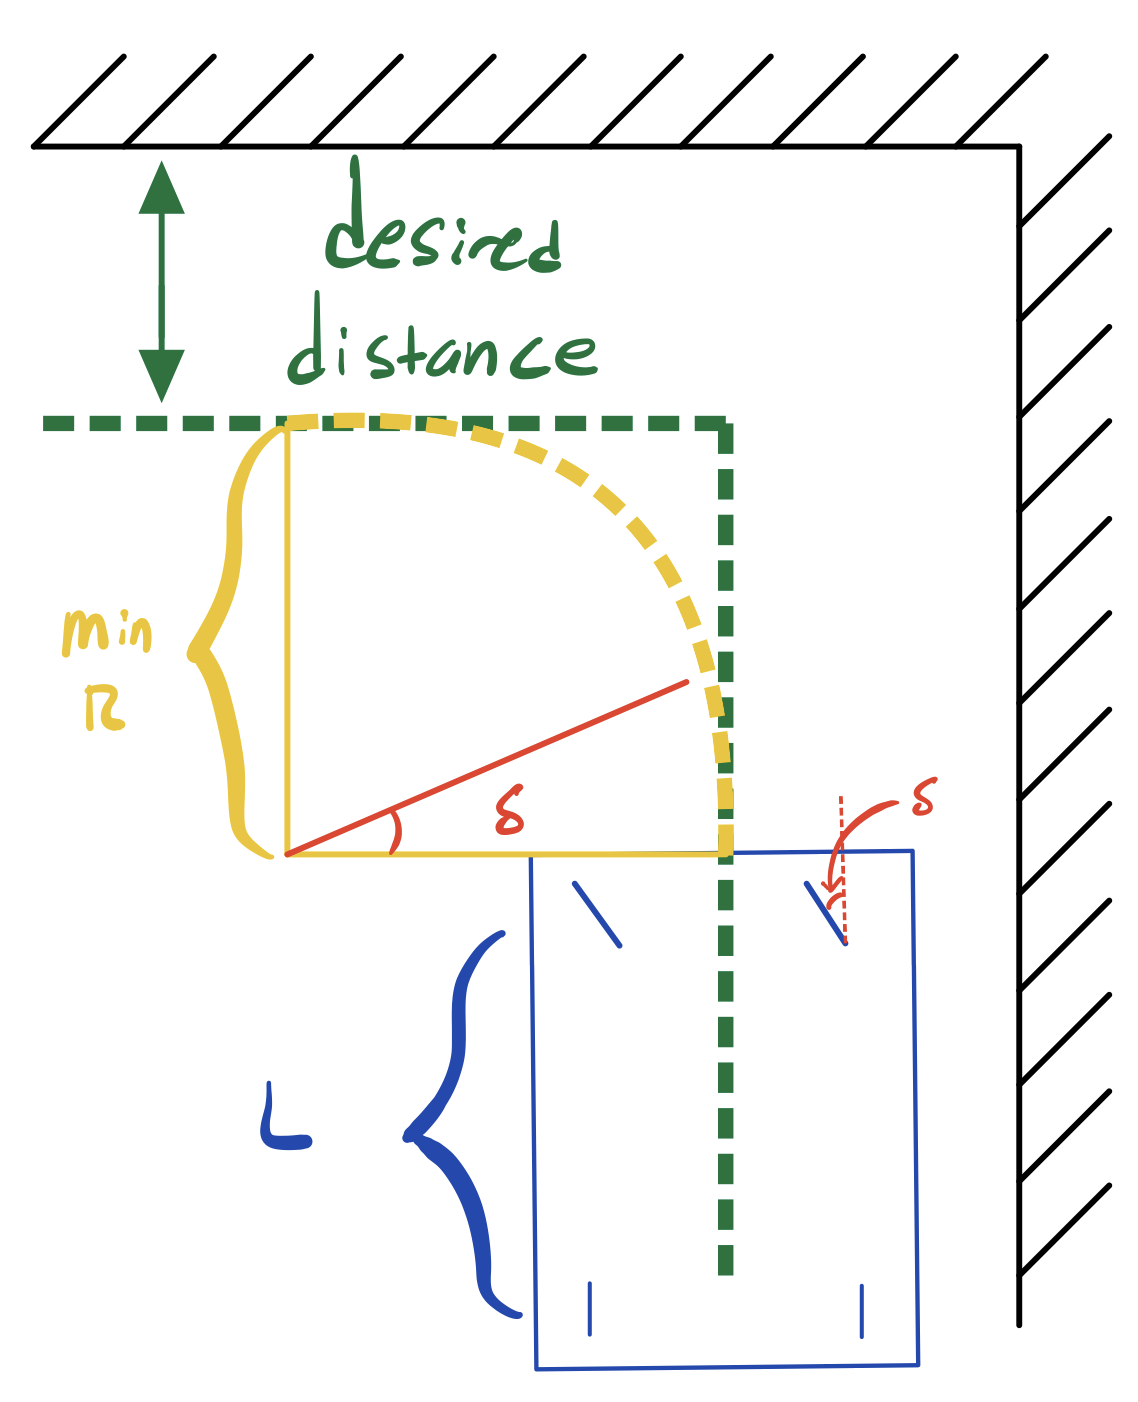
\includegraphics[width=0.5\textwidth]{imgs/min_r.png} % Include the image min_radius.png
\caption{The minimum turning radius is a function of the length between the two axles and the maximum steering angle of the car. Together they can be used to calculated R_{min}.}
\end{center}
\end{figure}

\subsubsection{ROS Implementation}
Written by: Marisa Hoosen\\

Running our code in ROS involved running a launch file with both the wall\_follower and safety\_mechanism nodes. Within the wall\_follower script, we accessed the LaserScan data by subscribing to the "scan\_topic." Our robot was controlled by publishing AckermannDriveStamped messages to the "drive\_topic", consisting of the velocity, acceleration, and steering\_angle\_velocity we wanted to assign to our robot. \\

We published Marker messages to the "visualization\_marker" topic to display the regression line our robot was aiming to follow. \\

Additionally, the params.yaml file was used to store the topic names and constants for a particular run, including the SIDE, VELOCITY, and DESIRED\_DISTANCE constants. We were able to easily change this file in between tests without having to make changes to the main file with the algorithm. \\

\subsection{Safety Controller}
Written By: Frank Gonzalez and Toomas Tennisberg\\

Our safety controller focuses on what is directly ahead of the car. If at least ten percent of the points detected within a 30 degree arc directly ahead of the racecar (from -15 degrees to +15 degrees in the car's frame of reference) are within a specified threshold, the car comes to a complete stop.\\\\
Our choice of a safety controller was determined by thinking about the situations in which the car might actively encounter a hazard. For our purposes, the only situations in which any safety controller could react appropriately is when the car is approaching an object or person directly ahead of it. Conducting experiments with our initial controller brought the conclusion that our safety controller should be parameterized on velocity. Specifically, the distance at which the car should shut off it's motors (stopping distance) needed to increase linearly with velocity. An equation governing the relationship between when the car should shut off its motors with respect to velocity is given in Equation 7:

\begin{equation}
    stopping\_dist \leftarrow -0.34 * v + final\_stop\_dist
\end{equation}

Our choice of angle was determined by balancing the field of view we provided to the car with the desired safety factor. We did some tuning to make sure that it did not accidentally stop in front of the wall when our intended action was to turn away from it.\\



\subsubsection{Safety Controller Integration}
Written by: Kaitlin Zareno\\

To get our safety controller integrated with our code, we published the safety controller to a mux thread that was higher up in the hierarchy than our wall following code. By having the safety controller higher in the hierarchy, the safety controller mechanism would be able to override the wall following code such that if a human or object became too close to the car during autonomous motion, the car would execute the safety controller over the wall follower. Highest in the hierarchy is teleop/manual control, which would allow the driver to regain manual control of the car regardless of the situation. This is necessary in case the safety controller or wall following code fails and human intervention is needed to safely operate the car.

\section{Experimental Evaluation}
\begin{comment}
The purpose of this section is to \textbf{provide evidence of the functionality} of your design, and to \textbf{document your experimental evaluation}. The section should explain both:

\subsection{Error calculation} 
To numerically judge the success of our wall follower, we calculated the overall and straight-wall error at each velocity. The mean error 

\begin{enumerate}
\begin{item}
\textbf{what} was tested and \textbf{why}, and \textbf{how} those tests were performed (Technical Procedures, including a clear definition of the performance metrics used in the analysis),
\end{item}
\begin{item}
and \textbf{discuss the result} of those tests to arrive at an assessment of the functionalities you implemented in this lab (Results).
\end{item}
\end{enumerate}

\textbf{You can find ideas and suggestions in the “Good Experimental Evaluation” Recitation on Canvas (Modules section).}\\\\
(no more than 1250 words)

\end{comment}

\subsection{Wall Follower PD Controller Evaluation}

\subsubsection{Error Collection and Visualization}
Written By: Zoe Wong\\

To evaluate the performance and robustness of our wall following algorithm, we measured the error when traveling at two different speeds (0.5 and 1.0 meters per second) along a path full of difficult corners and turns. The specific path traveled is illustrated in Figure 4. \\

\begin{figure}[h]
\begin{center}
\begin{tabular}{c c c c}
% (a) & 
% 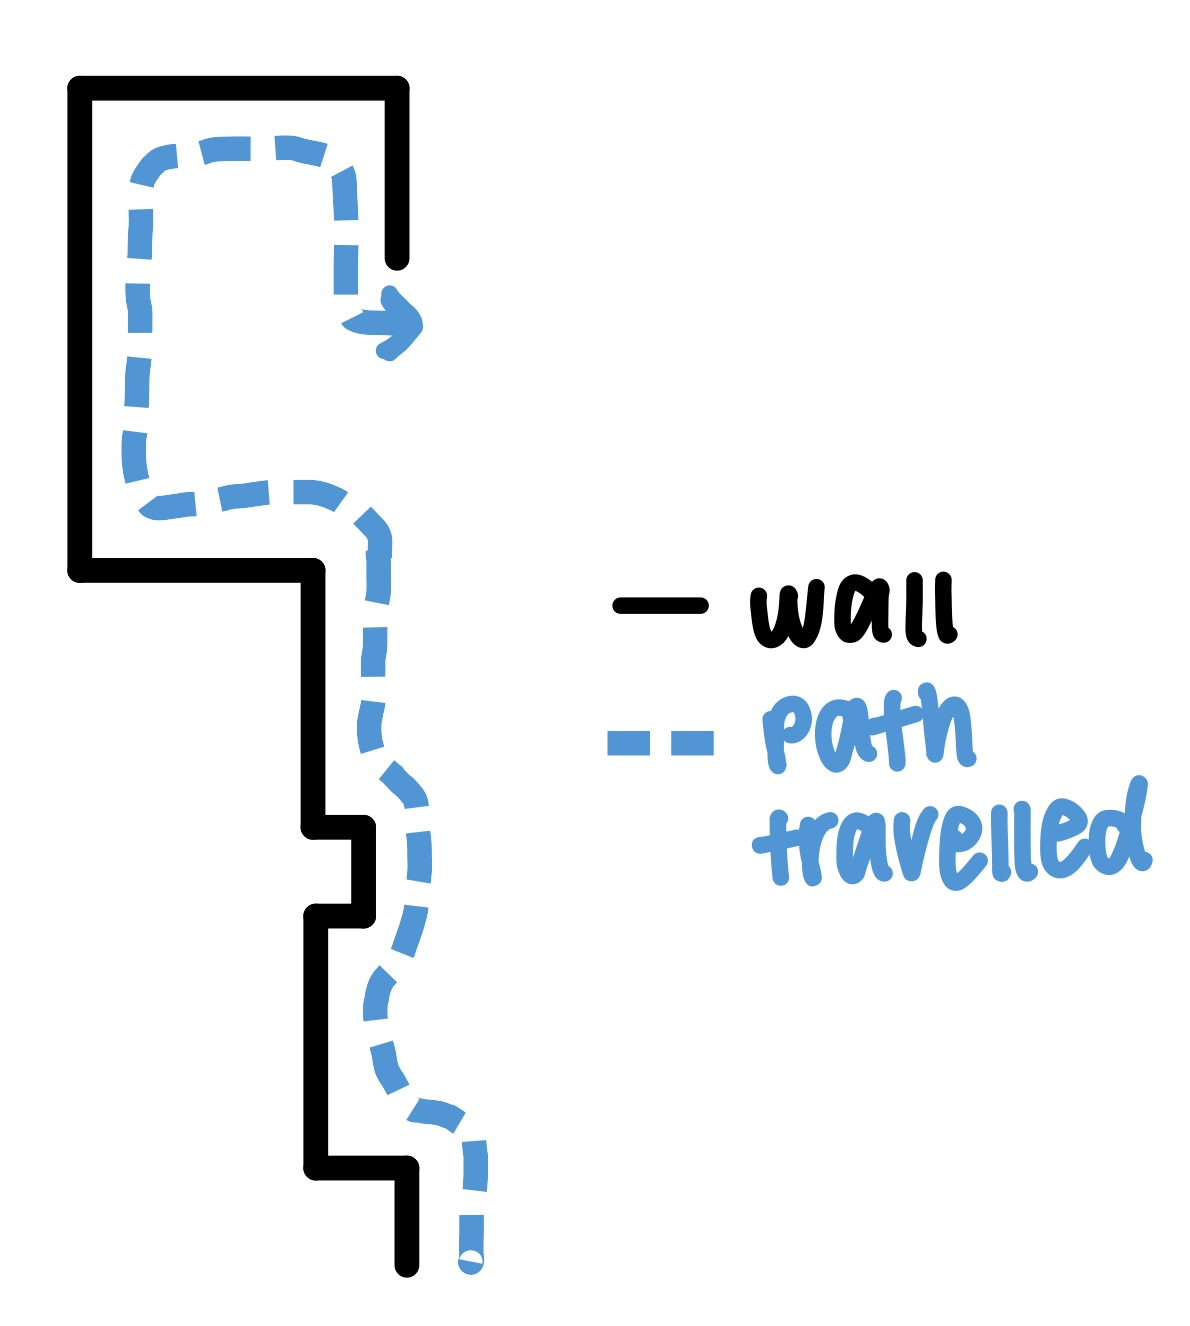
\includegraphics[width=.4\textwidth]{imgs/error_path.jpg} % Include the image placeholder.png
% &

% (b) & 
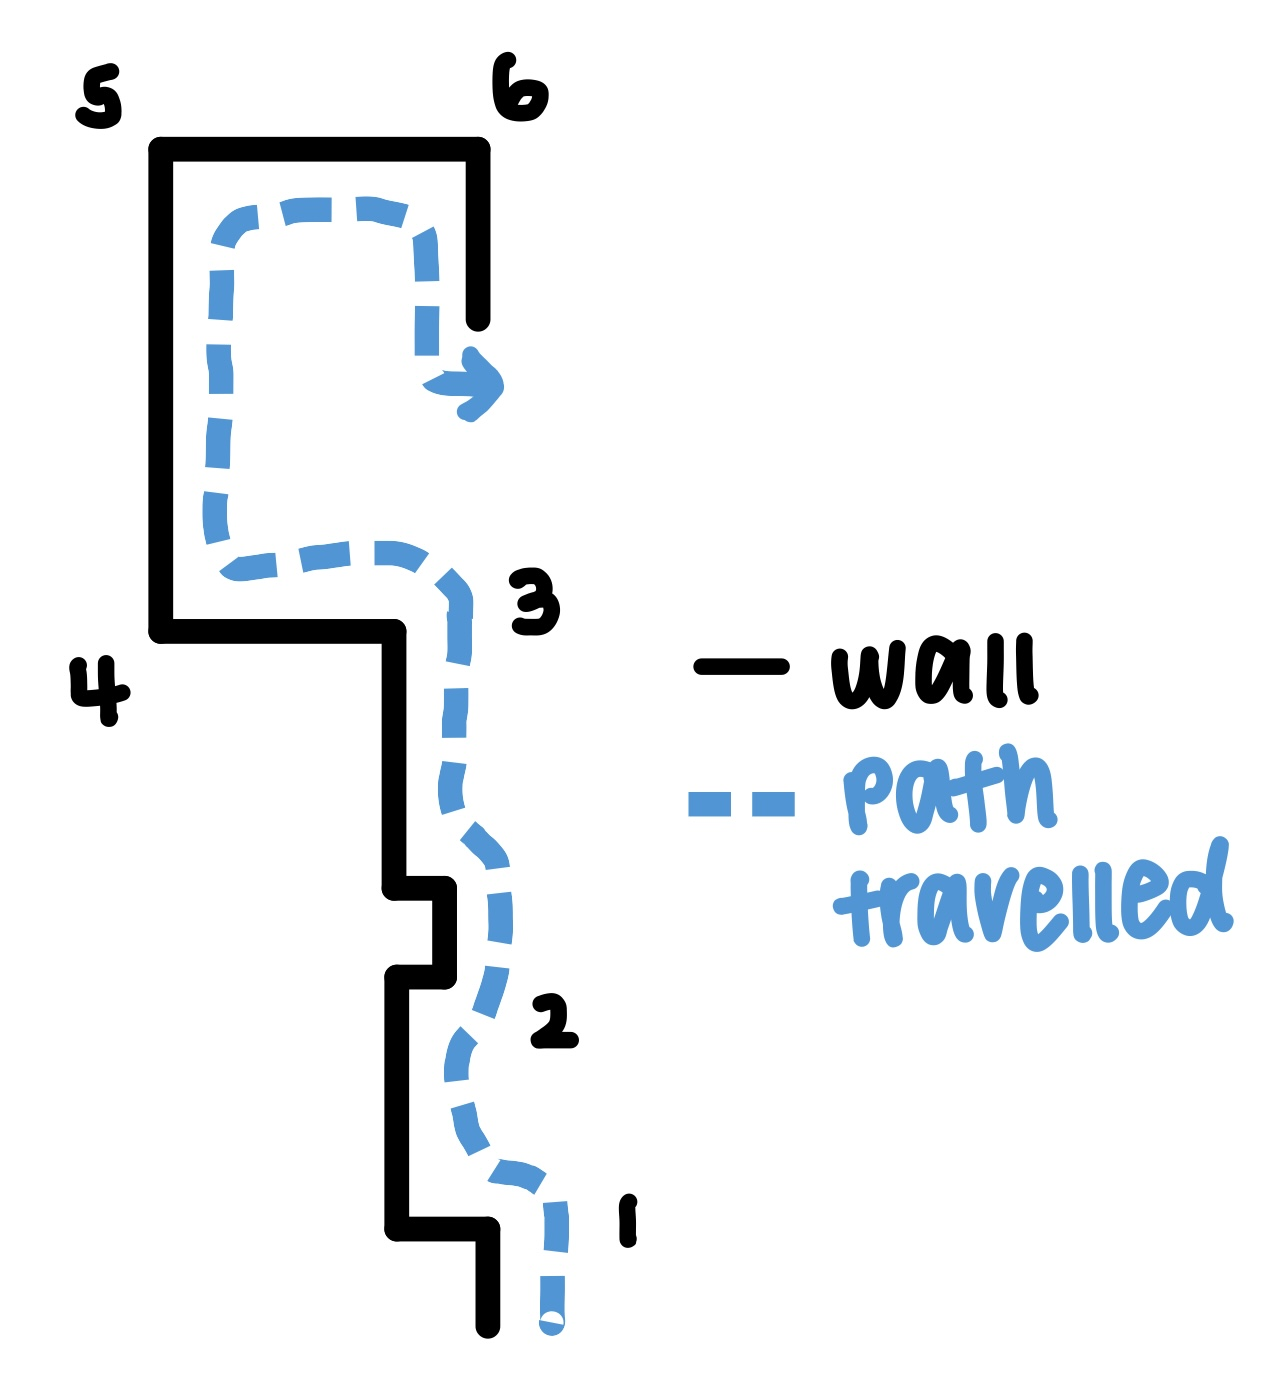
\includegraphics[width=.4\textwidth]{imgs/error_path_labeled.jpg} % Include the image placeholder.png
\end{tabular}
\caption{Path traveled during error collection, with numbers labeling the corners which correspond to the 6 peaks in the error plot shown in Figure 5.}
\end{center}
\end{figure}

In the PD controller, the error was defined as the difference between the minimum/perpendicular distance from the wall estimation and the desired distance away from the wall. For error collection, we published this computed error to an \texttt{"/error"} topic, whose messages were recorded as rosbags and logged into .txt files. The error data was then extracted, parsed from the .txt files, and plotted using the Python library \texttt{matplotlib}, creating the graph shown in Figure 4. \\

Since the robot travels along the path faster when the velocity is 1.0m/s and the period of each PD controller iteration was pretty consistent, there were also fewer messages compared to when the robot drove at 0.5m/s. For this reason, we graphed the error versus the relative location along the path traveled instead of time or the controller iteration. Given the same surroundings, we visually compared how well the wall-following PD controller worked at these two velocities. To determine the relative location, we defined the path distance as 100 meters and then evenly spaced the error messages for each velocity along the 100 meters since the robot was traveling at a constant velocity throughout. For example, a total of 761 error messages were created as the robot traversed through the path at 0.5m/s. Thus, we assumed that in each iteration, the robot traveled 100/761 $\approx$ 0.13 meters and computed its relative location accordingly. The relative location was defined as the iteration index $\times$ distance traveled per iteration. \\

We decided to compute our error intrinsically (based on the internal LIDAR measurements) because it would allow us to measure error with ease. However, by using intrinsic data, we did not account for cases where the wall estimations were not accurate in detecting the actual wall, such as corners. Thus, the computed minimum distance from the wall estimation was not always accurate in representing the actual distance from the wall. As an alternative, we could measure the error extrinsically by using a ruler to measure the physical distance between the robot and the wall. This method, however, could be prone to human error. Moreover, it would be difficult to measure this distance as the robot moves, especially at faster velocities. \\

\subsubsection{Error Analysis}
Written By: Zoe Wong\\

The blue and orange lines in Figure 4 represent the error measured when traveling at 0.5 and 1.0 m/s, respectively. Based on the graph alone, we could conclude that the error was a lot lower when traveling at slower velocities. Our computed values for the Total Mean Error, recorded in Table 1, supported this discovery. The Total Mean Error was defined as the average absolute value of the error along the entire path divided by the desired distance away from the wall, which was 0.5 meters in this case. When traveling 0.5 and 1.0m/s, this error was 16.6\% and 24.9\%, respectively. This analysis makes sense because when moving at slower velocities, the robot can readjust its position to the wall more frequently within the same distance traveled. Additionally, if we were to approximate the first derivatives of the error by finite differences, we would be able to see that the error derivative for 0.5m/s was closer to 0 than that for 1.0m/s, indicating that the wall follower controller's performance was also more stable and smooth at slower velocities. \\

\begin{figure}[h]
\begin{center}
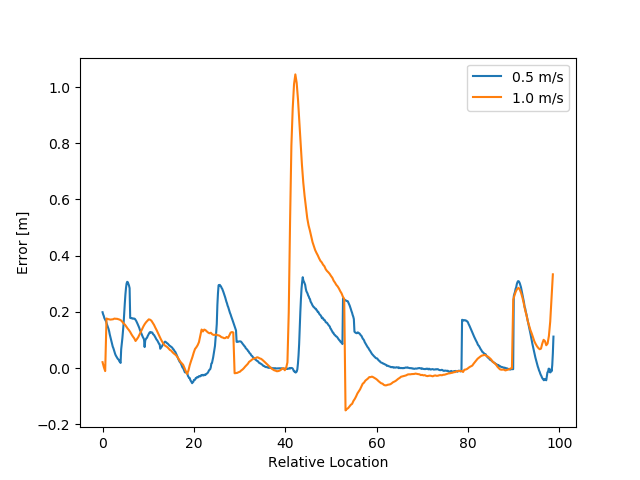
\includegraphics[width=.75\textwidth]{imgs/Error_graph.png} % Include the image placeholder.png
\caption{Error of actual distance to wall measured at $0.5$ and $1.0$ m/s on the path depicted by Figure 4.}
\end{center}
\end{figure}

\begin{table}[h]
\centering
\begin{tabularx}{0.8\textwidth} {
  | >{\centering\arraybackslash}X
  | >{\centering\arraybackslash}X
  | >{\centering\arraybackslash}X | }
 \hline
 Robot Velocity & Total Mean Error & Mean Error along Straight Walls\\
 \hline
 $0.5$m/s  & $16.6\%$  & $1.16\%$ \\
 \hline
 $1.0$m/s & $24.9\%$  & $6.89\%$  \\
\hline
\end{tabularx}
\caption{Computed mean errors at 0.5 and 1.0 m/s for the path depicted in Figure 4}
\label{tab:abc}
\end{table}

Additionally, after a thorough examination, the 6 error peaks noticed in the Figure 4 graph each indicate when the robot turned around a corner, labeled in Figure 3b. The robot was programmed to perform a hard turn if within a certain distance from the wall in front of it, a hard turn being a consistent max degree turn of .34 radians. The error spiked when turning around a corner because there is a moment when the robot is farther from the wall as it gradually turns away, as illustrated in Figure 5. As a result, the distances detected by the LIDAR would be greater and the wall estimation would be farther, thus increasing the error. \\

\begin{figure}[h]
\begin{center}
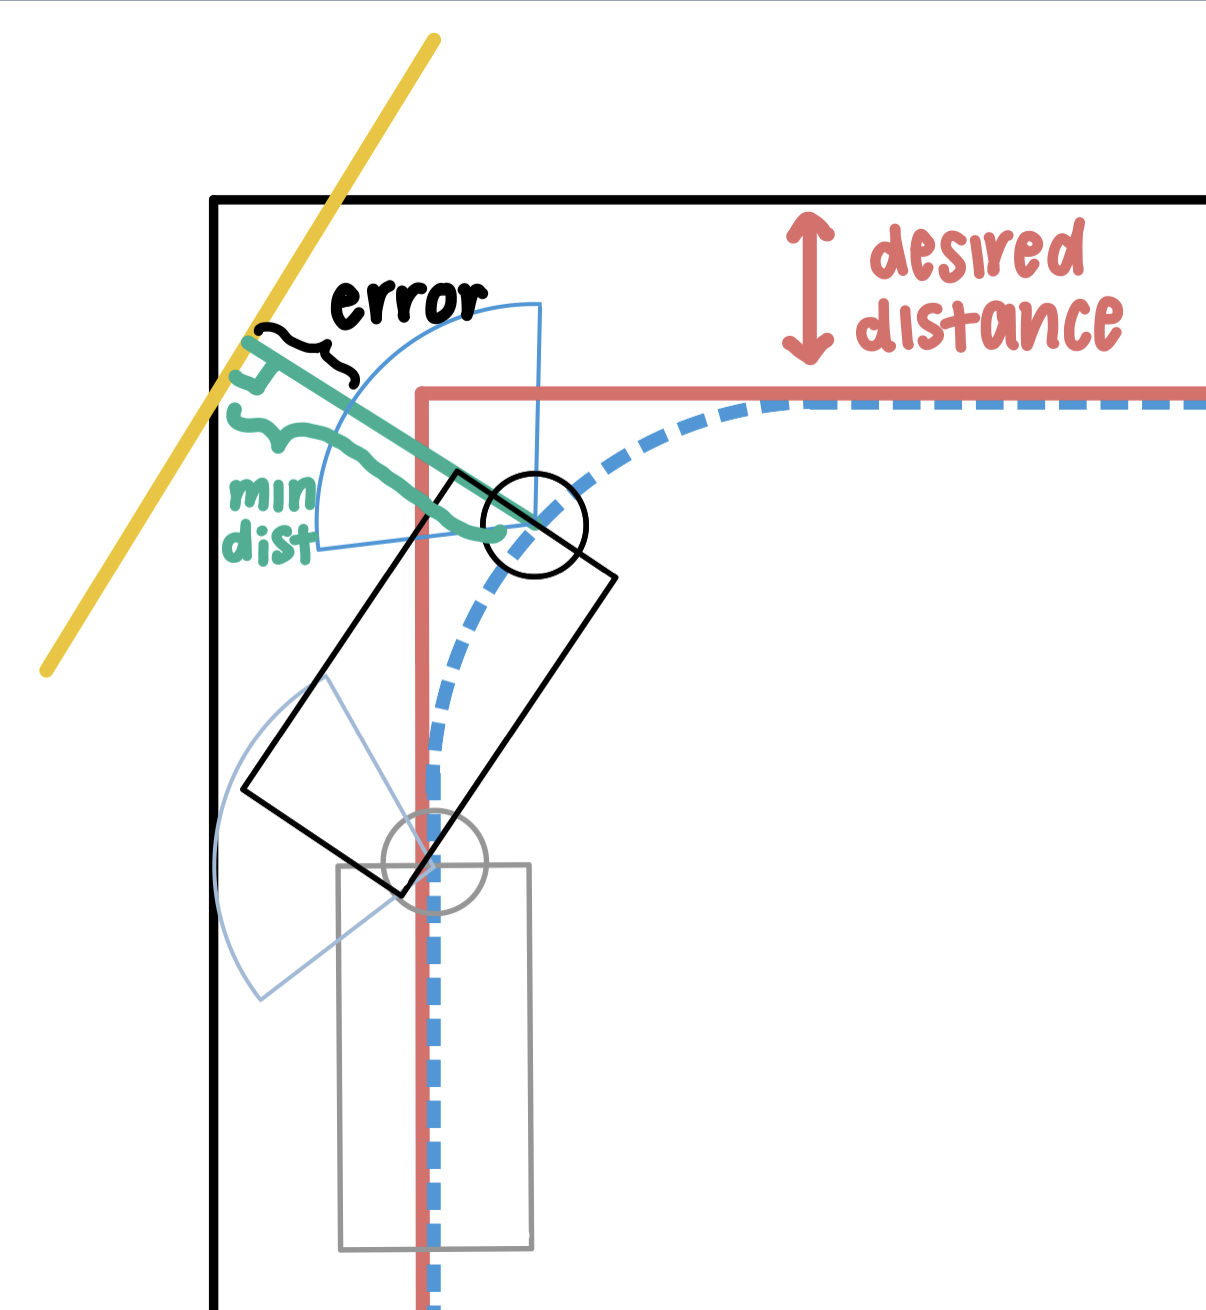
\includegraphics[width=.5\textwidth,trim={0 0 0 2cm},clip]{imgs/inner_corner.jpg} % Include the image placeholder.png
\caption{Visual representation of the error when turning in inner corner}
\end{center}
\end{figure}

The third peak is higher than other peaks because it is an outer/reverse corner. Before the robot detects an outer/reverse corner, it continues driving straight since a majority of the distances the LIDAR detects on the side are from the closer wall, making the wall estimation a good approximation, as illustrated in Figure 6a. Eventually, the robot overshoots the corner, and some of the detected side distances reflect off the farther wall. The wall estimation then adjusts itself by leaning towards the farther wall and reducing the slope, as shown in Figures 6b and 6c. Since the error was defined as the minimum perpendicular distance between the wall estimation and the robot, the error grows significantly during this adjustment of the wall estimation. In reaction to this adapted wall estimation and increased error, the robot turns into the wall estimation and eventually around the outer corner. \\

\begin{figure}[h]
\begin{center}
\begin{tabular} {c c c c c c}
(a) & 
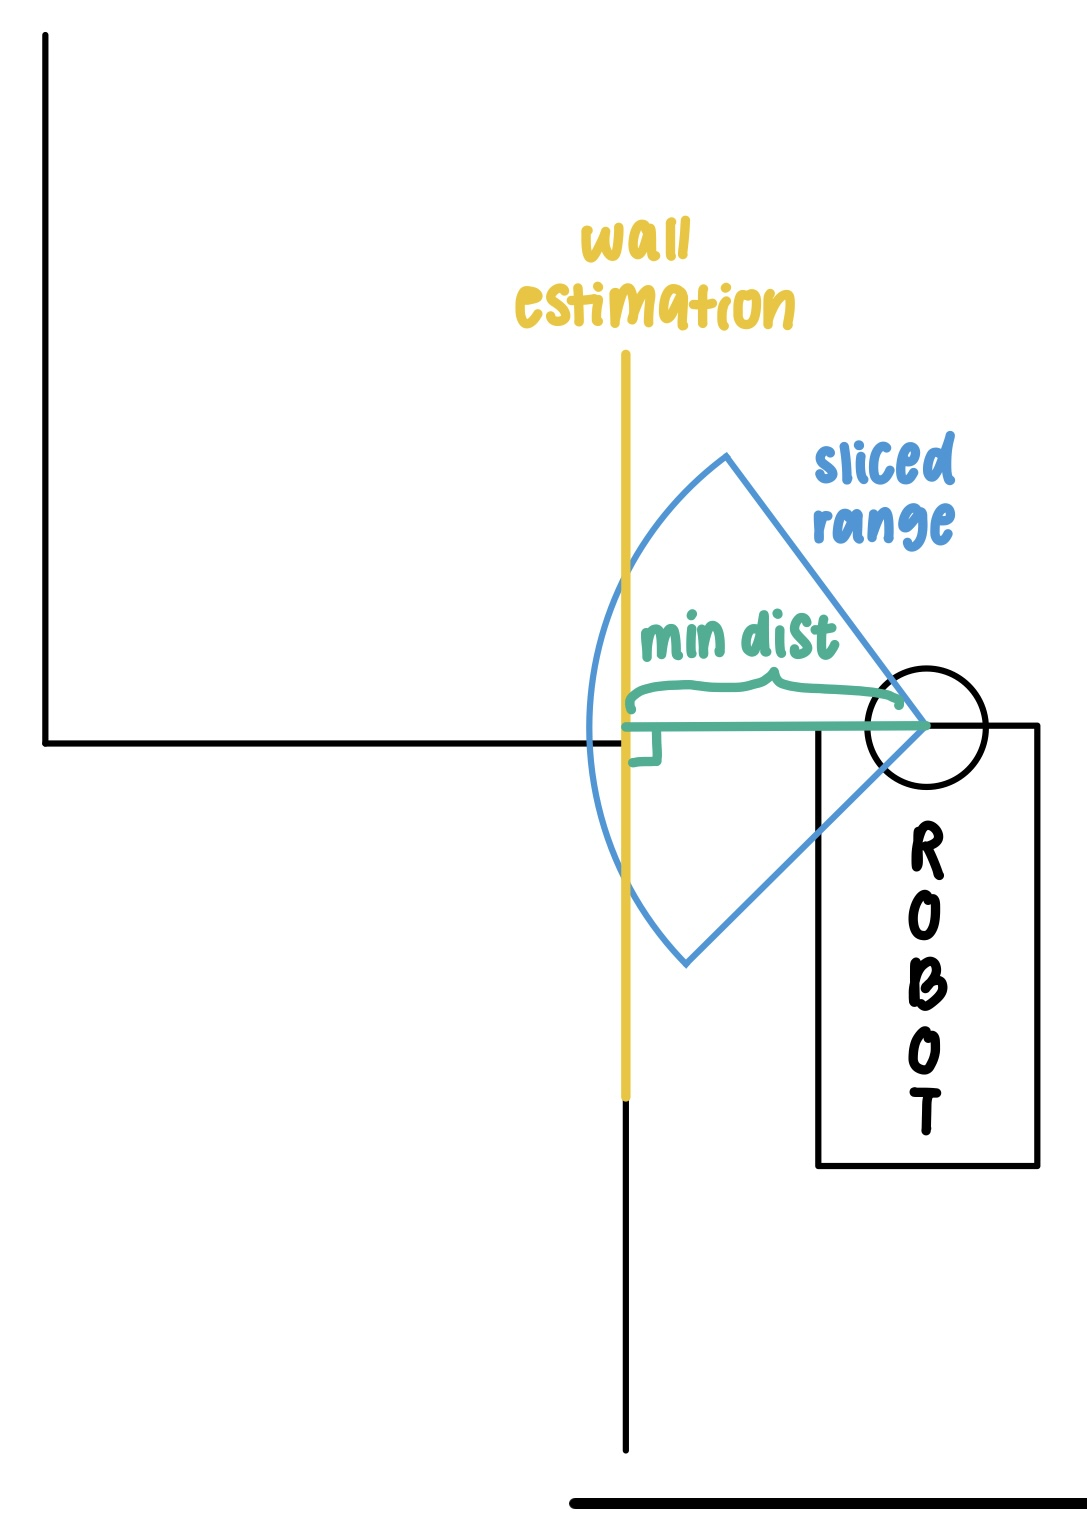
\includegraphics[width=.25\textwidth,trim={0 10cm 0 0},clip]{imgs/outer_corner_before.jpg} & 
(b) &
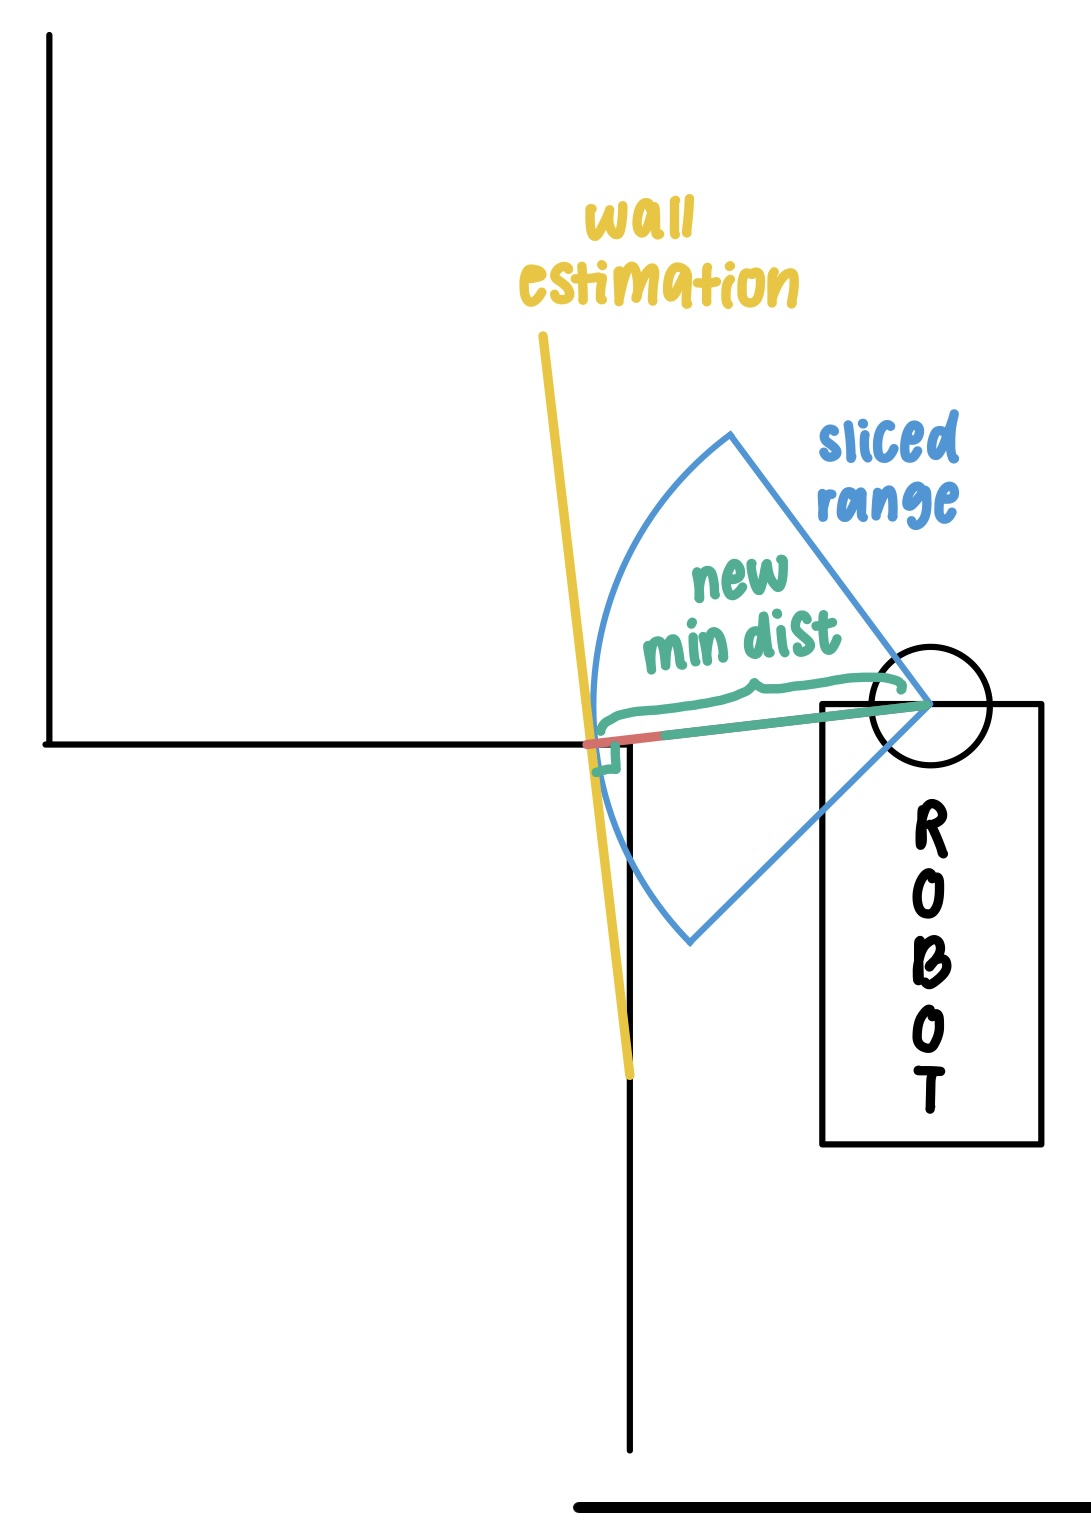
\includegraphics[width=.25\textwidth,trim={0 10cm 0 0},clip]{imgs/outer_corner_after.jpg} &
(c) & 
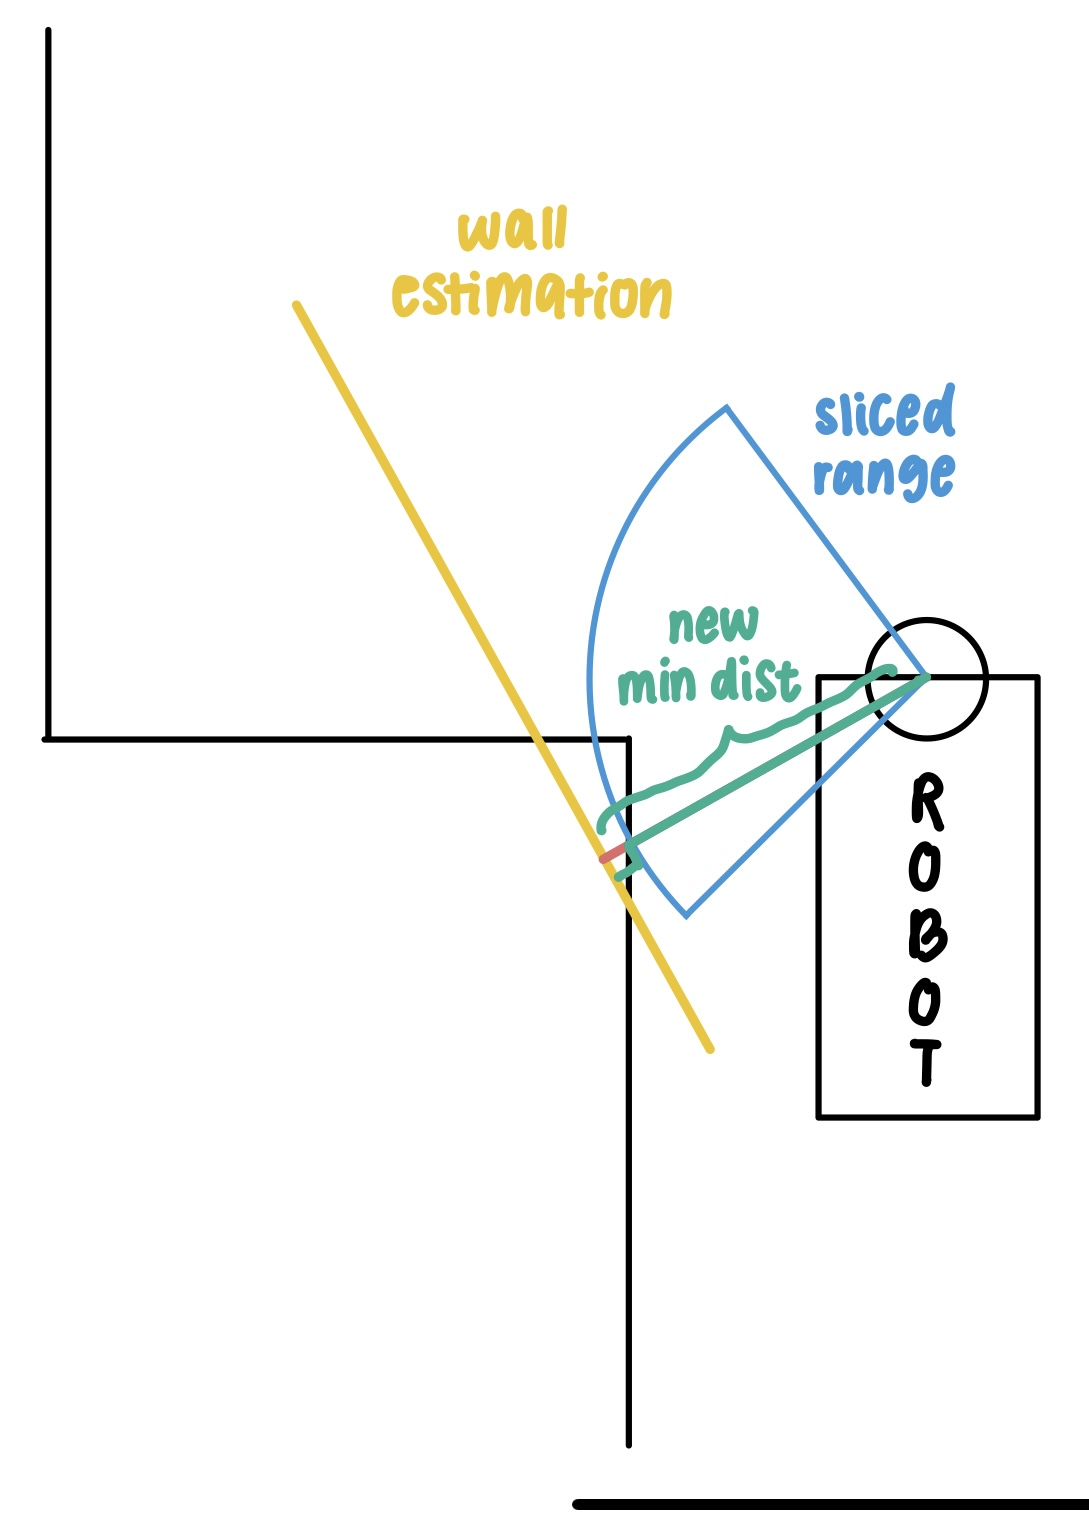
\includegraphics[width=.25\textwidth,trim={0 10cm 0 0},clip]{imgs/outer_corner_after_after.jpg} 
\end{tabular}
\caption{Visual representation of the error when turning around an outer corner}
\end{center}
\end{figure}

If we isolate and focus only on parts of the path where the robot is following a straight wall and not turning, we could see that the mean error for 0.5 and 1.0m/s are 1.16\% and 6.89\% respectively, as recorded in Table 1. Both are significantly less than their Total Mean Error, allowing us to conclude that the corners were a major contribution to the error. \\

\subsection{Safety Controller Evaluation}

\subsubsection{Error Collection}
Written By: Frank Gonzalez\\

To evaluate the performance of the safety controller, the vehicle was driven directly towards a wall at various velocities with a final stopping distance of 0.3 m. The actual distance at which the car stopped was recorded and the graphs in Figure 7 were generated from the data. 

\subsubsection{Error Analysis}
Written By: Frank Gonzalez\\

As shown in Figure 7, the car manages to always stop around the 0.35 m mark, providing a stopping error about 0.05 m. Given that the stopping error is positive, the car is being more cautious than we designed for, which we accepted over the alternative of not being cautious enough. It's worth mentioning the final data point, which had significantly more error. This is attributed to the last velocity test being conducted in a different environment, specifically the Stata basement floor rather than the RSS lab room. Since the floor is made of a different material, the deceleration rate would naturally change. Despite this change, the vehicle managed to still stop before colliding with the wall. This difference does however pose the question of whether the robot is robust enough to stop in an environment with a lower deceleration rate. In the future, testing in such an environment will be conducted. 

\begin{figure}[h]
\begin{center}
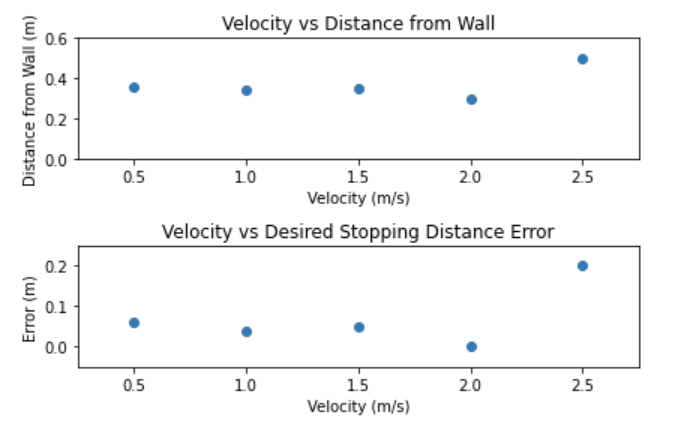
\includegraphics[width=.75\textwidth]{imgs/Safety_controller_error.png} % Include the image placeholder.png
\caption{Plot of velocity compared to distance from wall and error of desired distance}
\end{center}
\end{figure}

\section{Conclusion}
Written By: Toomas Tennisberg\\

\begin{comment}
Summarizes what you have achieved in this design phase, and notes any work that has yet to be done to complete this phase successfully, before moving on to the next. May make a nod to the next design phase.\\\\
(no more than 500 words)\\\\
\end{comment}

Over the past week, we have successfully implemented both a controller that follows a wall and a safety controller. The wall-following controller has a total mean error of 16.6\% at 0.5 {m/s} and 24.9\% at 1 {m/s}, but this is mainly due to the corners it encounters. The mean error among straight walls is 1.16\% and 6.89\% respectively. While these results are satisfactory for us, they could be improved upon by using a better linear regression algorithm, like RANSAC or MSAC, adding an integral term to the controller, and/or tuning the controller values with more testing.\\\\ 
The safety stop controller successfully halts the robot with 0.05m error with starting velocities ranging from 0.5 to 2.5 m/s, though the final result is dependent on the environment. Further experiments are needed to conclude how the controller should be modified to account for these environmental changes. We should also ensure that the safety controller does not impede on the normal operations of the robot. While the current design works for the purposes of wall following, changes might be needed if the robot becomes too cautious in the future. \\\\


\section{Lessons Learned}
\begin{comment}
Presents individually authored self-reflections on technical, communication, and collaboration lessons you have learned in the course of this lab.
\end{comment}

\subsection{Frank Gonzalez}
On the technical side, the most important lesson I learned was how important is it to start early and have a contingency plan for when things go wrong. Originally, everything was moving smoothly: the code was uploaded on the car, recordings were made, and it seemed that the team would be smooth sailing for the rest of the lab. Then, unexpectedly, the algorithm we were using ceased to function, and despite our best efforts, debugging the issue became an impossible task, even with instructor aid. Despite the setback, we had means of moving forward: the other wall following codes that hadn't been selected to go on the car. Luckily, the newly selected code functioned well and we were able to redo our recording and collect additional needed data.\\

As for communication, I learned the importance of effective and clear communication with my teammates. As a team, we worked very well during this lab with no conflicts and a clear direction as to what we were working towards. Such a dynamic was thanks to everyone's ability to communicate with each other and express their thoughts and opinions in appropriate manners, as well as people's willingness to accept feedback and criticisms on their proposed ideas. \\

Lastly, collaboratively, splitting the team to work on different components massively accelerated the rate at which we managed to complete our tasks. Had we instead all worked together on making a website, then prepping the robot, then the presentation, and then the report, we most likely would've had a much harder time finishing our goals on time. In splitting up the work however, things happened at a much faster and smoother pace. \\

\subsection{Marisa Hoosen}
In the technical aspect, I learned the importance of error analysis and having a good way of testing if our solution actually does a good job of accomplishing our intention. Analyzing our own data can also help debug exactly where something is going wrong, and problem-solve to find a solution. \\

Working to make our slides easily understandable and clear was necessary to our presentation. I learned that it was better to rely on diagrams and video to visualize a point while talking about how it functions as opposed to having all slides be bullet points. I also realized how it was important to make points stand out and use the slides to supplement our presentation, rather than it being the bulk of our point. \\

Our communication and planning for this first lab worked out very well. By planning meetings out in advance and coordinating responsibilities, we were able to stay organized and on top of the work we had to do. Starting early was also very useful, giving us time to readjust our wall following algorithm when we ran into bugs with our previous method. Keeping an active group chat helped us to stay updated and knowledgeable about our progress. \\

Collaboration-wise, bouncing ideas between each other helped us not get stuck to a particular idea or method, allowing us to weigh the benefits and drawbacks of specific methods. Working in pairs or smaller groups at times also helped to be able to have a few focused on a smaller part of the challenge, but also have more than one part of the process moving forward at once. \\


\subsection{Toomas Tennisberg}

On the technical side, my main takeaway was the amount of effort needed to balance the safety controller with the wall follower. One of our earliest test runs was at 0.5m/s and the robot managed to do a full lap around the classroom before we realized that the safety controller was buggy and not actually working. When we got it fixed, the car just refused to take any corners because the safety stop mechanism engaged too aggressively. The current safety controller appears to maintain this balance however.\\\\
From a communication standpoint, I learned how to sell my ideas to my teammates, and also how to write and present our work. Communication was mostly smooth in our team, mostly due to good delegation and consensus on larger issues, so the biggest hurdle that we had was making our point clear to an audience.\\\\
For collaboration, the biggest lesson I learned was to sanity check. There was a bug in a teammate's code and we had no idea why the error acted the way it did. So I looked at it and realized it wasn't doing what it was supposed to be doing, which allowed them to fix it and we got the nice clean error metrics that can be seen in the final result.

\subsection{Zoe Wong}

On the technical side, the main lesson I took away from this lab was to be open-minded because there could be many different approaches to the same problem. I was fascinated when I first heard how other teammates implemented their wall-following algorithms. For example, one teammate applied distance-dependent weights to reduce the impact of farther points when using linear regression for wall estimation. I also heard some others regarded points that were more than twice the desired distance away from the robot as outliers and removed them completely during wall estimation. To provide another example, while I applied a hard turn to prevent the robot from crashing, another member adapted the LIDAR scan data ranges to include corner points when within a certain distance from the front wall to adapt the wall estimation to account for corner cases. Through our brainstorming of ideas, I was able to learn from their different approaches and improve on my own. Additionally, this lab had emphasized that simulation is indeed very different from the real-life. When we first tested the wall-following algorithms and controller constants we wrote for simulation on the robot with velocity set as 1.0m/s, we witnessed severe oscillation, which sometimes triggered the safety controller. The constants that worked in simulation did not work as well in reality, which makes sense because there are many factors that are not accounted for in simulation, including friction. \\

When it came to communication, I was impressed by our team's effective and clear communication since the very first team meeting, where we each tried to sell our wall-following algorithm to other teammates. Whenever there were misunderstanding or confusions, our members asked and answered immediately. With our shared willingness to communicate and work together, we were able to select an algorithm that satisfied everyone and started working with the robot during our second meeting. Communication also played a key role when debugging each other's code. To locate a bug, it was effective to talk it out with members so that they could understand and potentially help with the issue, or so we could notice bugs in our logic. For this reason, I am thankful for our team's ability to share ideas with and accept feedback from the team, because if not for that, our project may not have went as smoothly as it did. In addition to teamwork, communication was important when explaining our project during the briefing. From this experience, I learned how diagrams and full-sentence titles can significantly help the audience understand the point we are trying to make. \\

For collaboration, the most significant takeaway I got from this lab was that we should start as early as possible and stay on top of deadlines. Given that everyone has their own schedules, it could always be hard to find time when everyone is free to work together. Thus, it would be best to divide tasks as soon as possible so members could work on their parts on their own time before a rare team meeting to ensure we work efficiently. By starting early, we had time for potential setbacks, including testing and debugging, which could take a long time. While pure teamwork was sufficient, I believe it would also be important to have a leader figure in our team, responsible for planning group meetings, reminding members of upcoming deadlines, checking up on everyone's progress, and guiding team discussions. The leader would help the team work efficiently and smoothly, without problems. During this lab, it was nice how this role seemed to rotate among our team members, depending on how busy everyone was. \\

\subsection{Kaitlin Zareno}
On the technical side, my main takeaway was the necessity of sanity checks. This was especially important when updating our safety controller. Although we had an initial idea of what we wanted the new  controller to do, it was good to actually go though the math step by step to make sure that what we were doing was logical and explainable. In addition, another thing that I learned was how important it is to start the technical work early—we started working on the robot over the weekend and this gave us the flexibility to pivot/make changes when unexpected bugs came up.\\

With respect to communication, I learned the importance of effective and concise communication with my teammates. I also learned how important it is to keep the conversation flowing; sometimes the group would be neutral on an idea or be stuck on something for a while and it was important for someone to help move the team’s conversation forward in order to allow us to converge on a viable solution. Lastly, I learned how to more clearly express my thoughts to an audience through graphics and informative (not overwhelming!) PowerPoint slides.  \\

Collaboration-wise,  I learned the importance of setting expectations for when to meet a as group and using our time together in person as efficiently as possible. Planning to meet on the weekends and delegating responsibility allowed us to break down the problem into more manageable subsections. This is crucial and is something that will be more important in the future, especially when we increase the amount of technical work we do in the week. In addition, setting expectations for the team/team culture allowed us to work better as a group, as it put everyone on the same page with respect to what was expected technically and socially from each member (and hopefully will foster a healthy team environment). 

\begin{comment}
\section{Formatting examples for figures, pseudocode, etc}

\subsection{Tables}

Many other table packages and options exist but here is one example:\\\\

\begin{tabularx}{0.8\textwidth} {
  | >{\raggedright\arraybackslash}X
  | >{\centering\arraybackslash}X
  | >{\raggedleft\arraybackslash}X | }
 \hline
 item 11 & item 12 & item 13 \\
 \hline
 item 21  & item 22  & item 23  \\
\hline
\end{tabularx}

\subsection{Images}

\begin{figure}[h]
\begin{center}
\includegraphics[width=0.65\textwidth]{placeholder} % Include the image placeholder.png
\caption{Figure caption.}
\end{center}
\end{figure}

\subsection{Code Blocks and Algorithm Pseudocode}

% Including Python code blocks:

\begin{lstlisting}
json
{
  "6.141": "normal",
  "16.405": "woke",
  "no_sleep": "spoke"
}

def do_something_productive():
  if not_productive:
    do_work()
  else:
    cry()
\end{lstlisting}

% Using the algorithm2e package for pseudocode:

\begin{algorithm}[H]
\SetAlgoLined
 \While{alive}{
  \eIf{sleepy}{
   sleep\;
   }{
   eat\;
  }
 }
 \caption{caption}
\end{algorithm}

% Using the algorithmic package for pseudocode:

\begin{algorithmic}
\STATE $i\gets 10$
\IF {$i\geq 5$}
        \STATE $i\gets i-1$
\ELSE
        \IF {$i\leq 3$}
                \STATE $i\gets i+2$
        \ENDIF
\ENDIF
\end{algorithmic}
\end{comment}

\end{document}
